%%CAP 1
\begin{figure}[h]
\includegraphics[width=\textwidth]{cap_1/es4/es4.png}
\caption{Esercizio 1.4}
\label{es14}
\end{figure}

\begin{figure}[h]
\includegraphics[width=\textwidth]{cap_1/es6/es6.png}
\caption{Esercizio 1.6}
\label{es16}
\end{figure}

\begin{figure}[h]
\includegraphics[width=\textwidth]{cap_1/es13/es13.png}
\caption{Esercizio 1.13}
\label{es113}
\end{figure}

%%CAP 2
\begin{figure}[h]
\includegraphics[width=\textwidth]{cap_2/es7/compar}
\caption{Comparazione del numero di iterazioni necessarie per i vari metodi}
\label{compar}
\end{figure}

%%CAP 4
\begin{figure}[h]
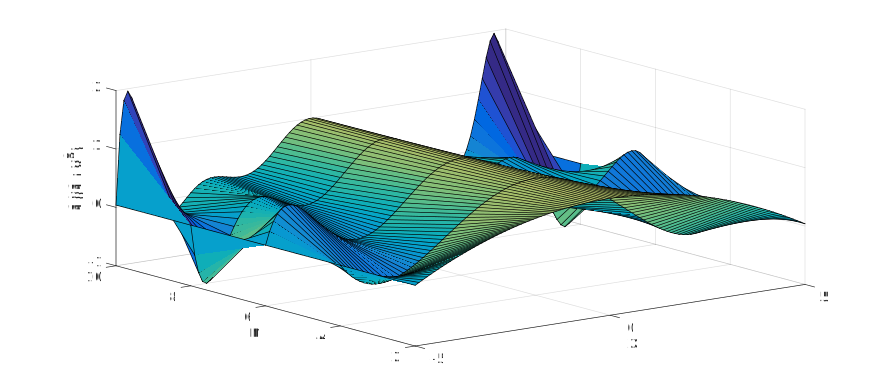
\includegraphics[width=\textwidth]{cap_4/es2/Runge_equi.png}
\caption{Ascisse Equidistanti per $f(x) = \frac{1}{1+x^2}$}
\label{RungeEq}
\end{figure}

\begin{figure}
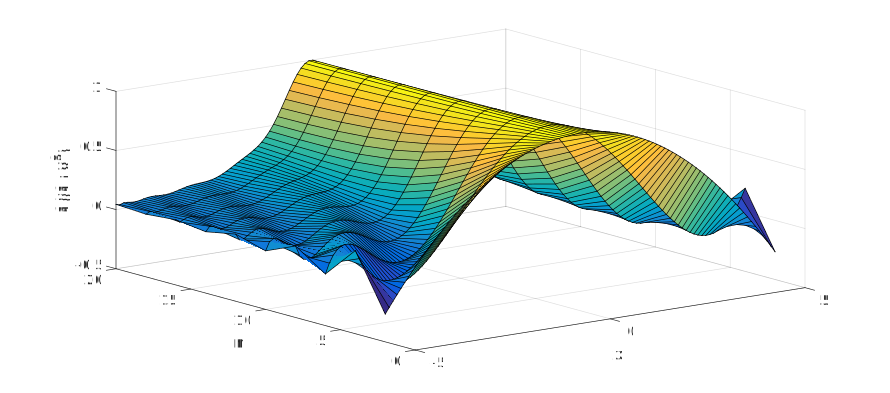
\includegraphics[width=\textwidth]{cap_4/es2/Runge_cheb.png}
\caption{Ascisse di Chebyshev per $f(x) = \frac{1}{1+x^2}$}
\label{RungeChe}
\end{figure}

\begin{figure}
\includegraphics[width=\textwidth]{cap_4/es2/Sin_equi.png}
\caption{Ascisse Equidistanti per $g(x) = sin(x)*x$}
\label{SinEq}
\end{figure}

\begin{figure}
\includegraphics[width=\textwidth]{cap_4/es2/Sin_cheb.png}
\caption{Ascisse di Chebyshev per $g(x) = sin(x)*x$}
\label{SinChe}
\end{figure}

\begin{figure}
\includegraphics[width=\textwidth]{cap_4/es2/Runge_equi_err.png}
\caption{Errore per Ascisse Equidistanti per $f(x) = \frac{1}{1+x^2}$}
\label{RungeEqErr}
\end{figure}

\begin{figure}
\includegraphics[width=\textwidth]{cap_4/es2/Runge_cheb_err.png}
\caption{Errore per Ascisse di Chebyshev per $f(x) = \frac{1}{1+x^2}$}
\label{RungeCheErr}
\end{figure}

\begin{figure}
\includegraphics[width=\textwidth]{cap_4/es2/Sin_equi_err.png}
\caption{Errore per Ascisse Equidistanti per $g(x) = sin(x)*x$}
\label{SinEqErr}
\end{figure}

\begin{figure}
\includegraphics[width=\textwidth]{cap_4/es2/Sin_cheb_Err.png}
\caption{Errore per Ascisse di Chebyshev per $g(x) = sin(x)*x$}
\label{SinCheErr}
\end{figure}

\begin{figure}
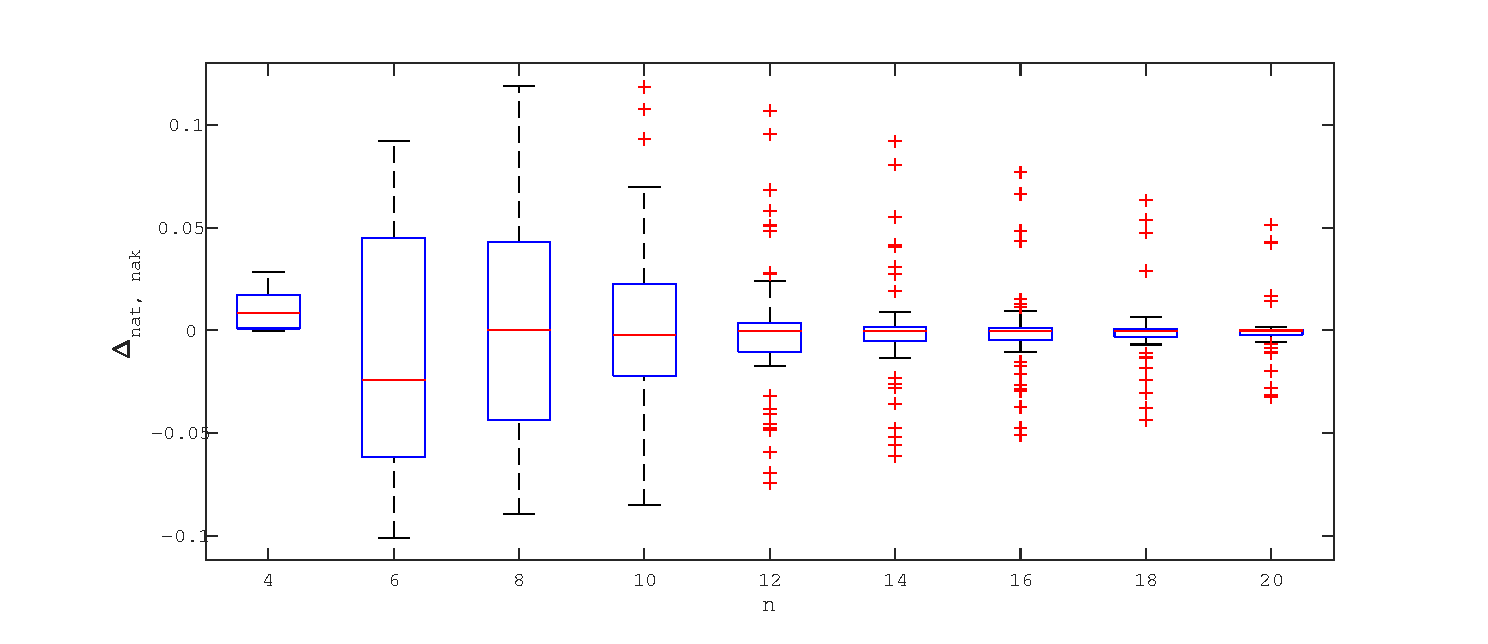
\includegraphics[width=\textwidth]{cap_4/es5/errors}
\caption{$\Delta_{nat, nak}$ per la funzione di Runge}
\label{err_runge}
\end{figure}

\begin{figure}
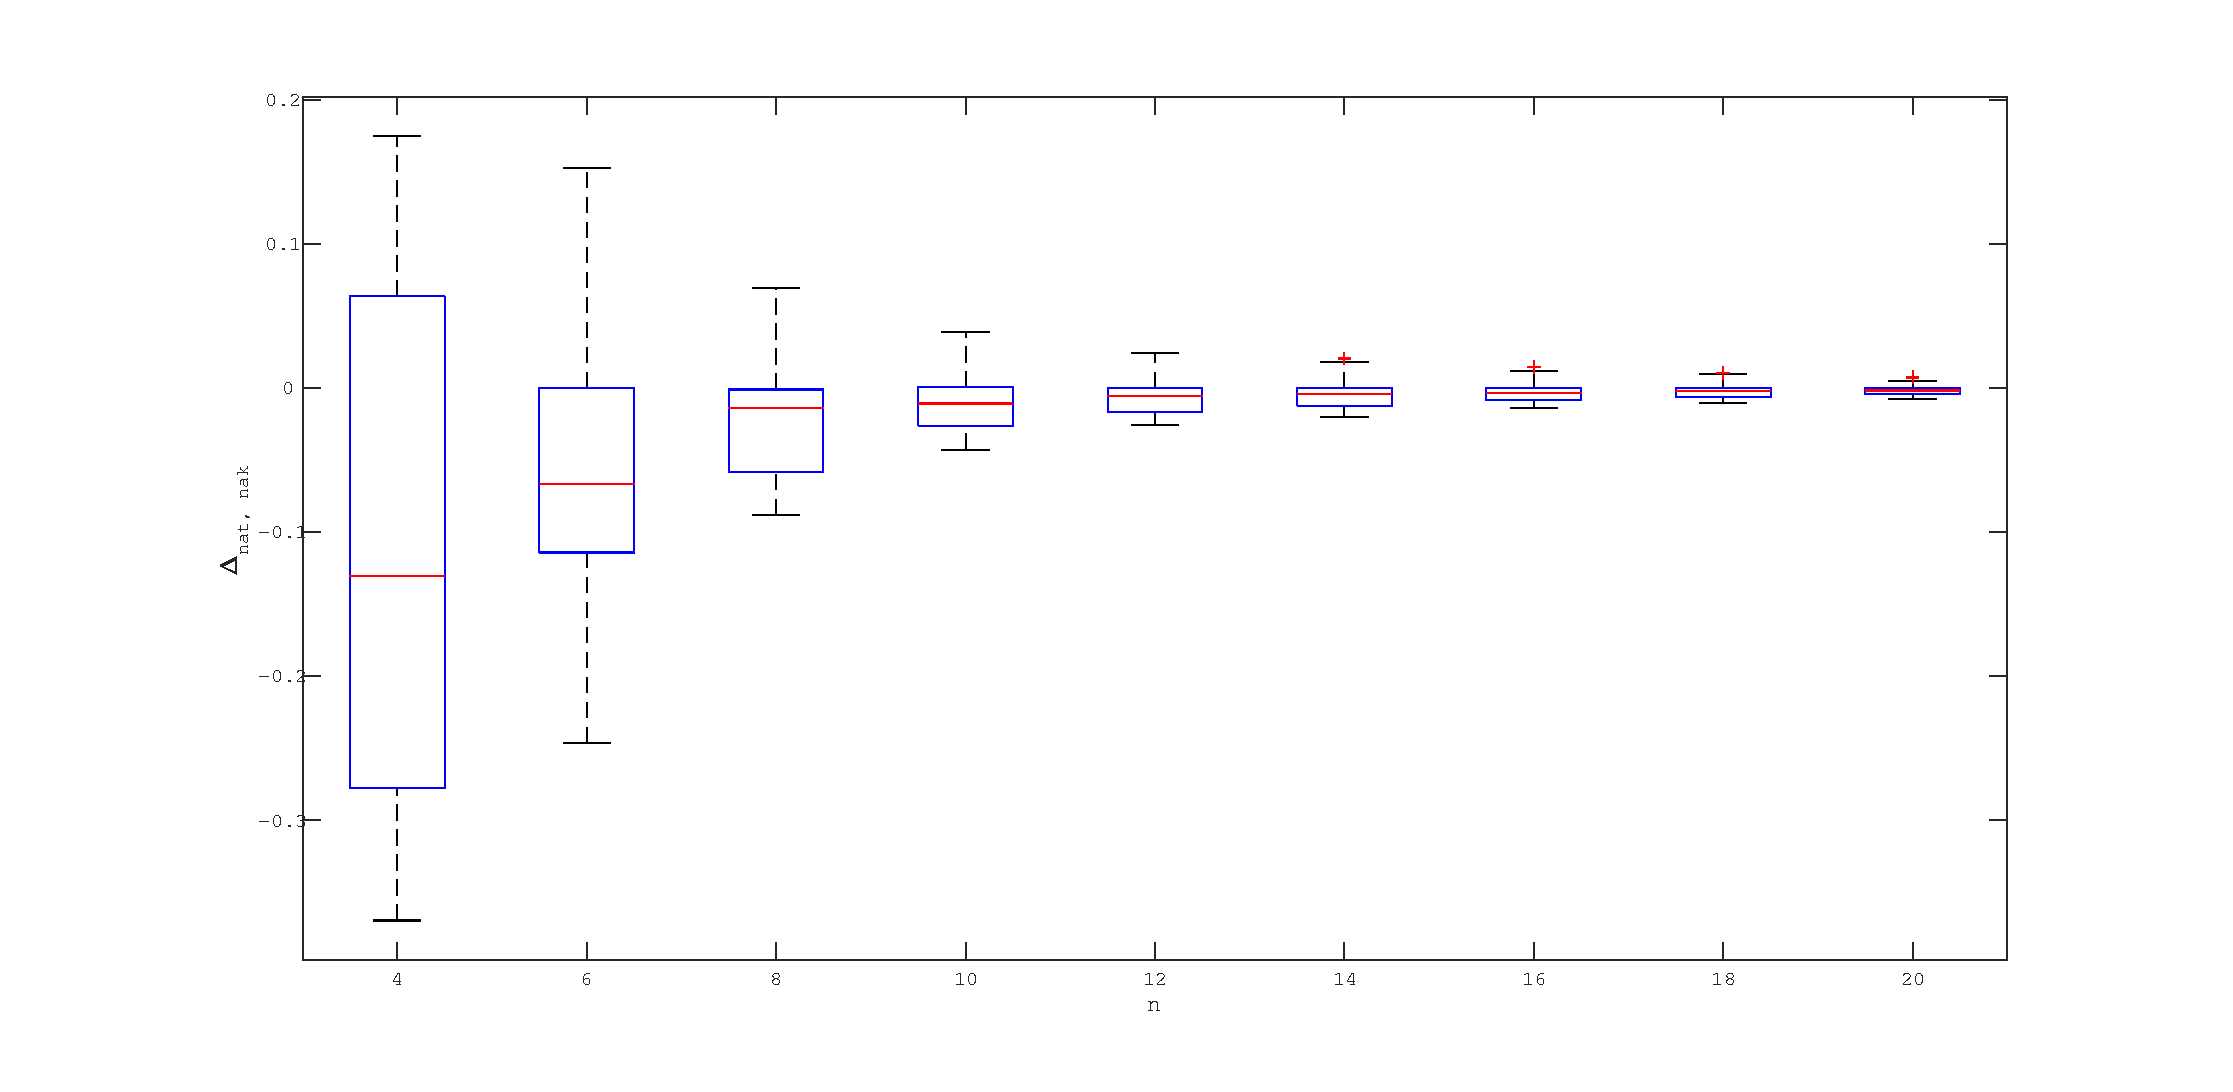
\includegraphics[width=\textwidth]{cap_4/es5/errors_sin}
\caption{$\Delta_{nat, nak}$ per la funzione $xsin(x)$}
\label{err_sin}
\end{figure}

\begin{figure}
\centering
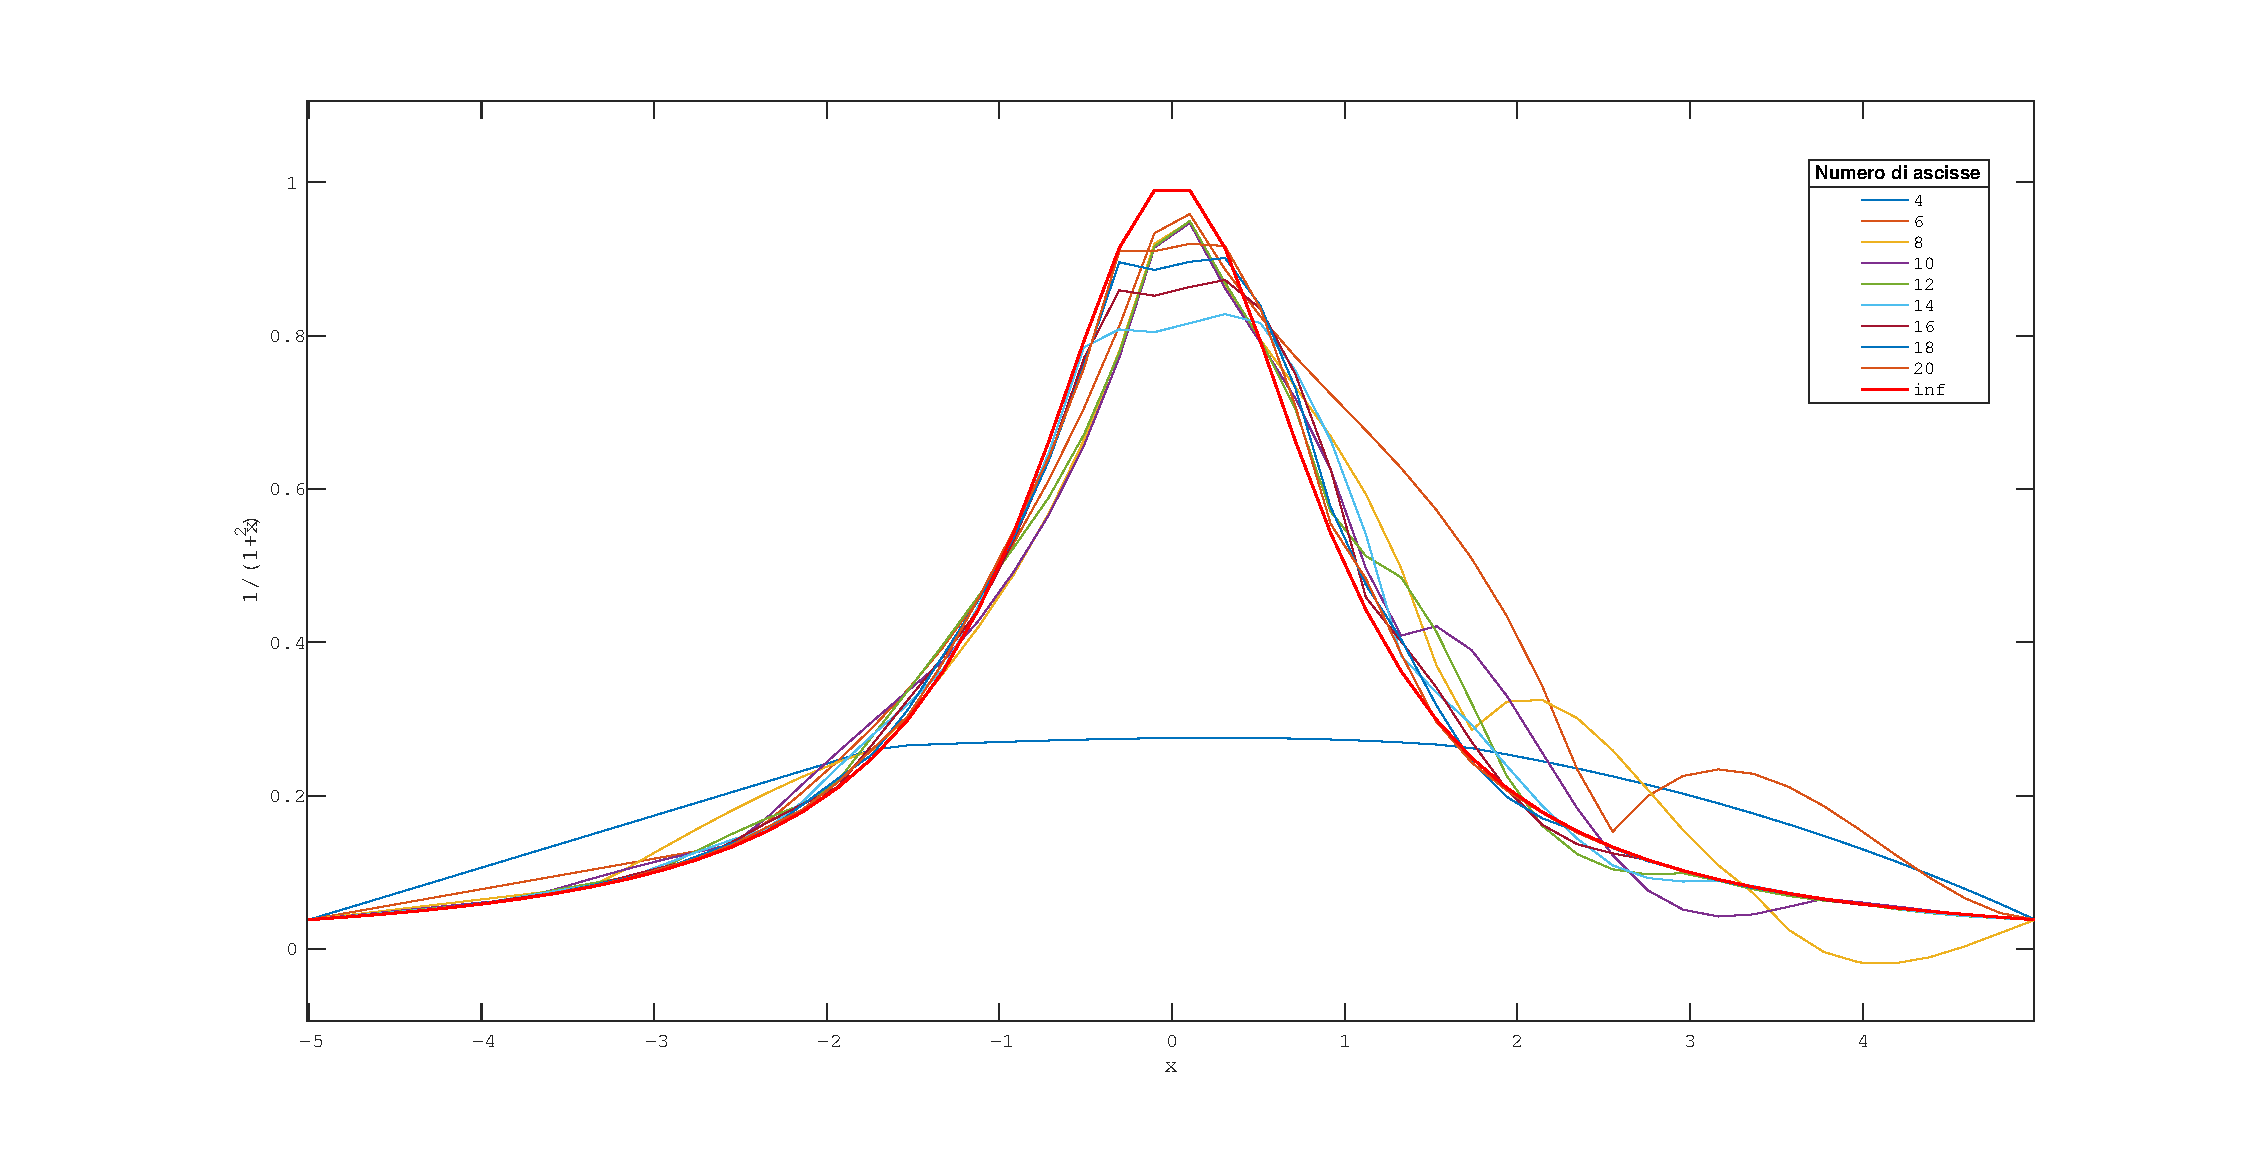
\includegraphics[width=\textwidth]{cap_4/es5/runge_nat}
\caption{$\frac{1}{1+x^2}$ interpolata con spline naturale}
\label{plot_runge_nat}
\end{figure}

\begin{figure}
\centering
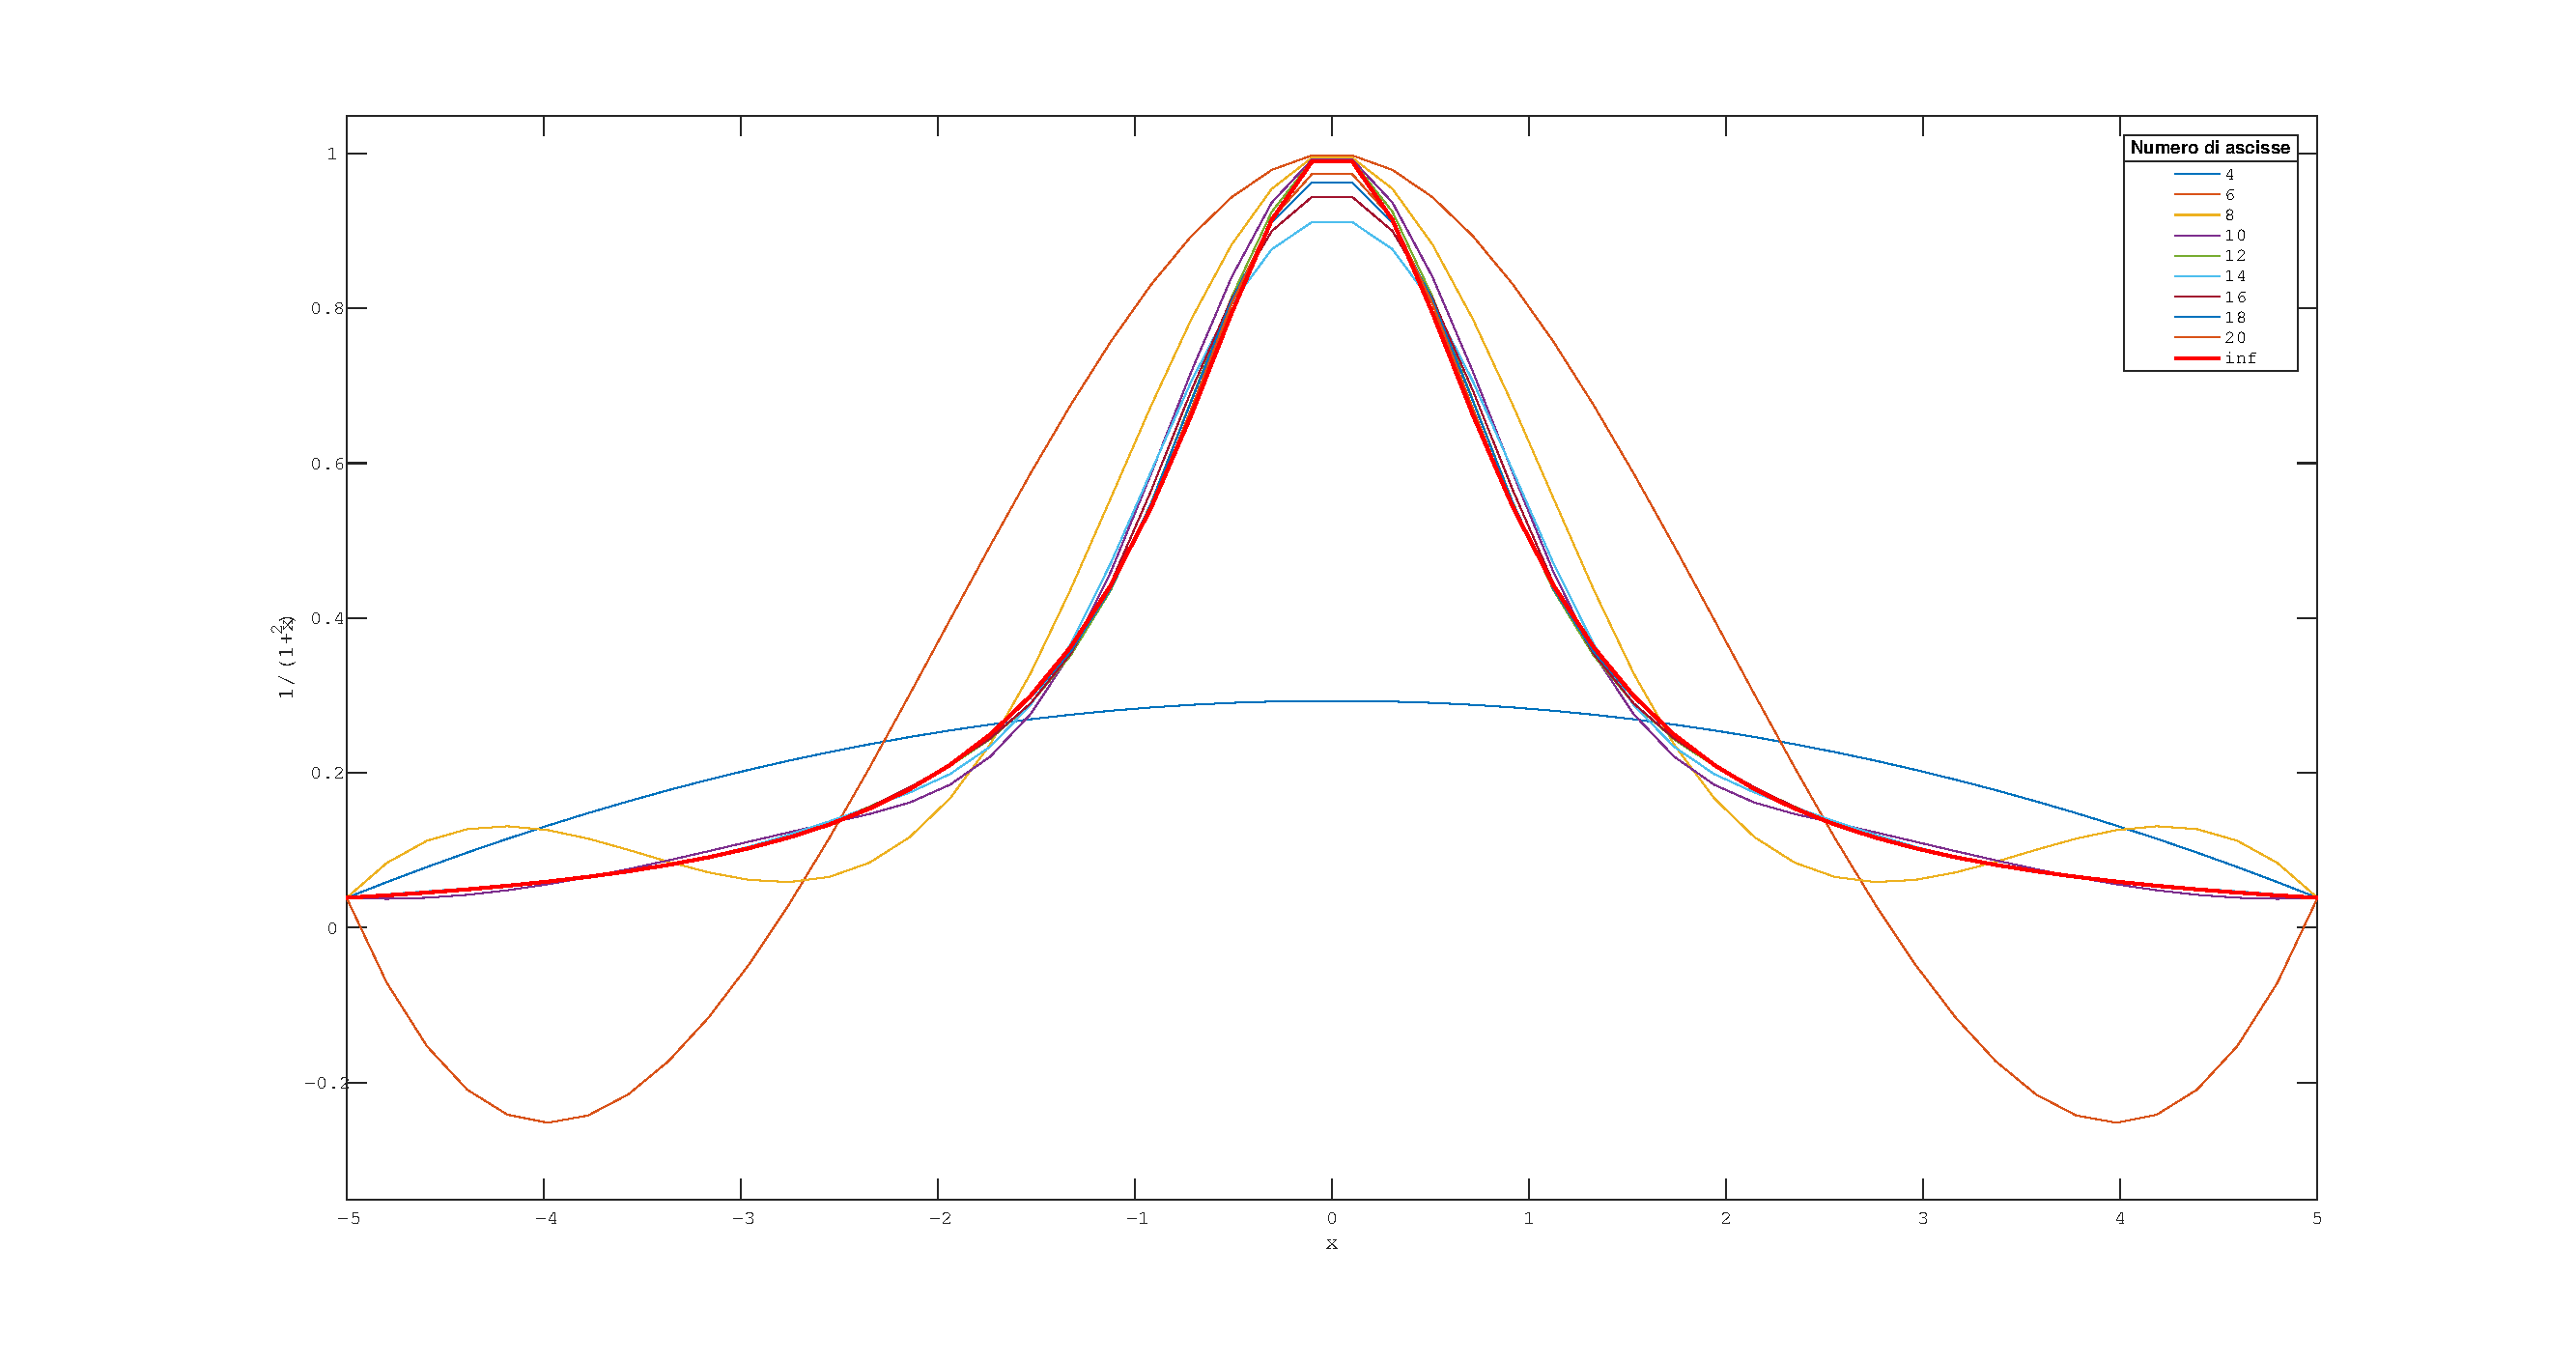
\includegraphics[width=\textwidth]{cap_4/es5/runge_nak}
\caption{$\frac{1}{1+x^2}$ interpolata con spline not-a-knot}
\label{plot_runge_nak}
\end{figure}

\begin{figure}
\centering
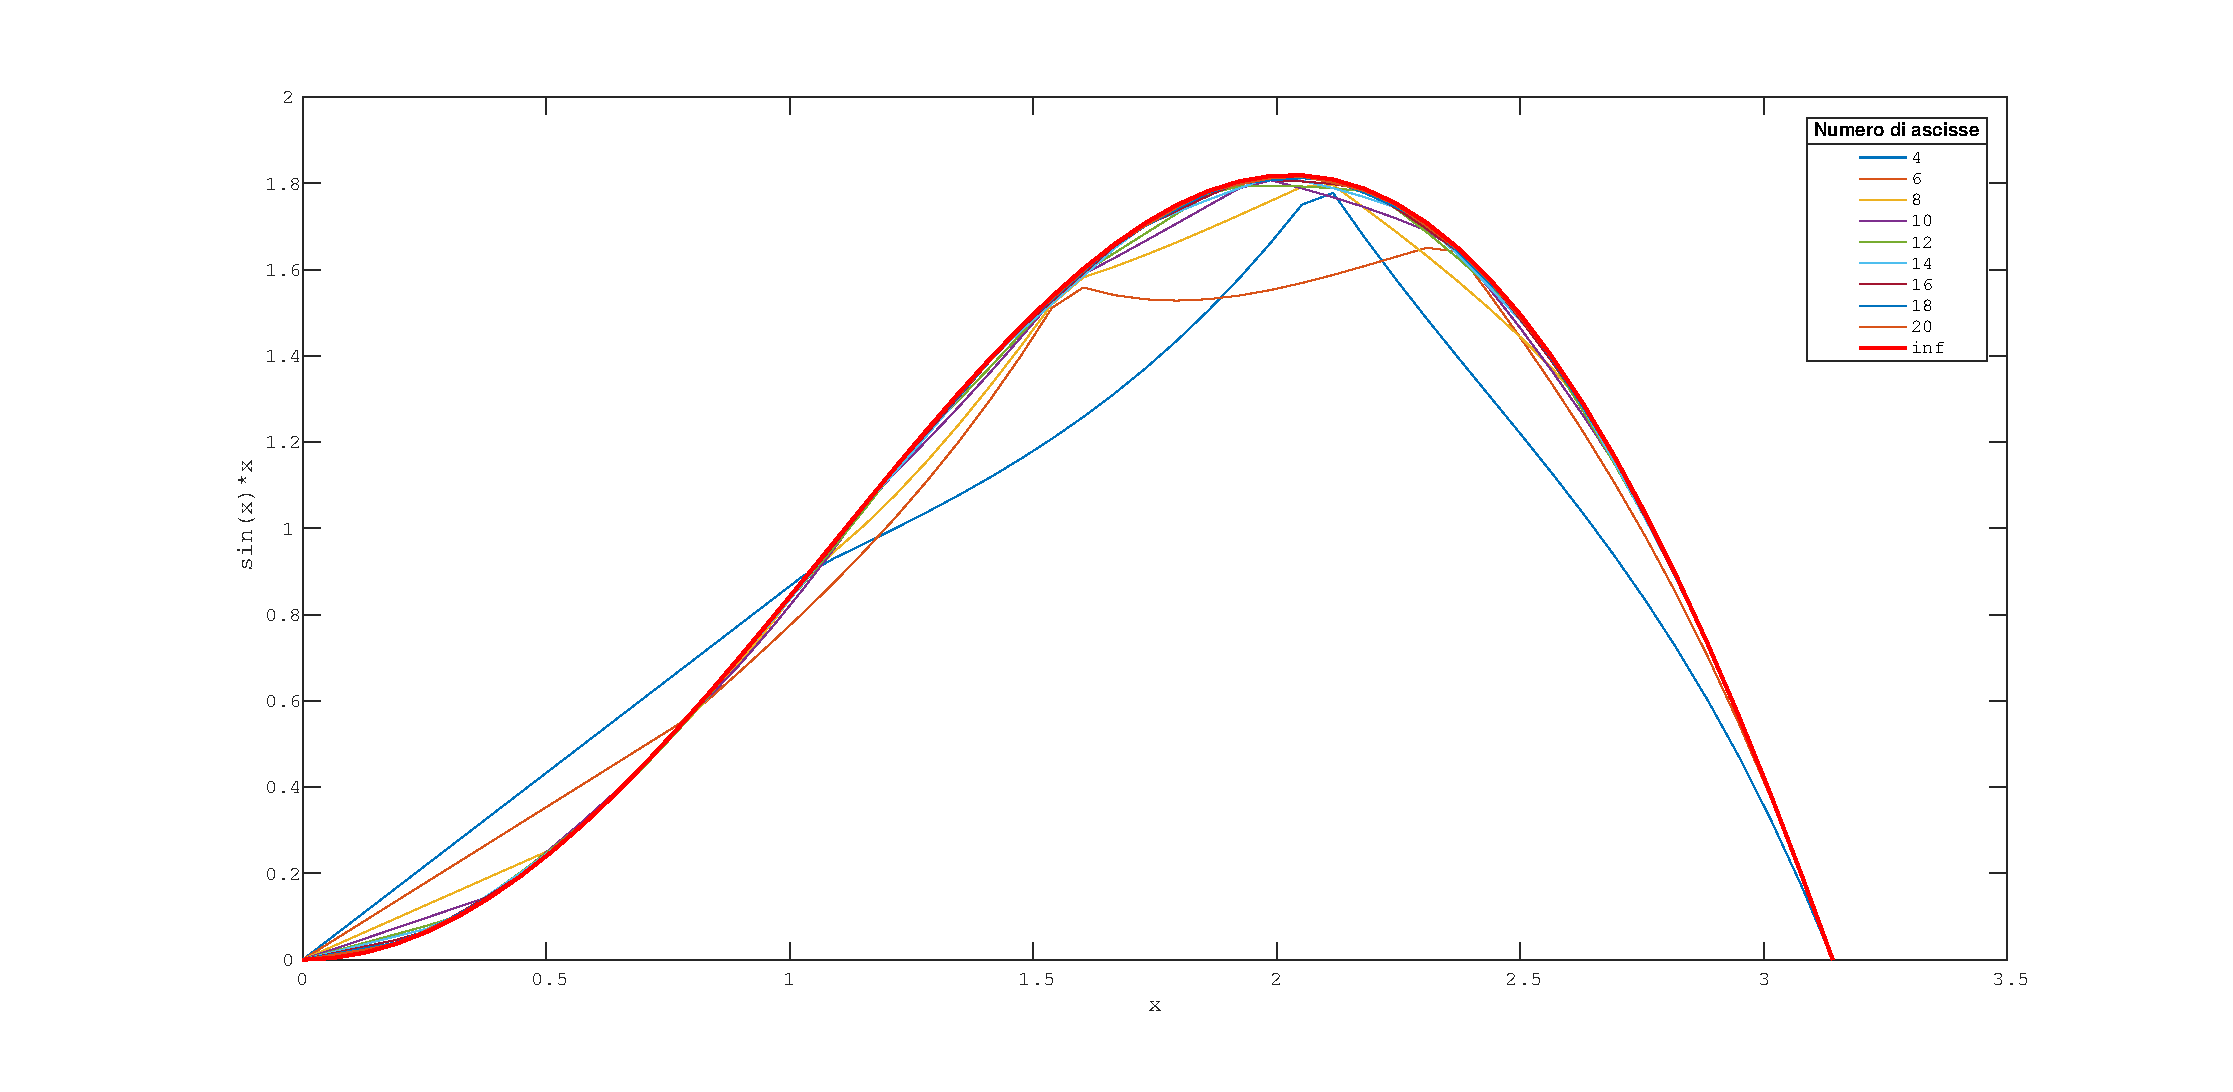
\includegraphics[width=\textwidth]{cap_4/es5/sin_nat}
\caption{$xsin(x)$ interpolata con spline naturale}
\label{plot_sin_nat}
\end{figure}

\begin{figure}
\centering
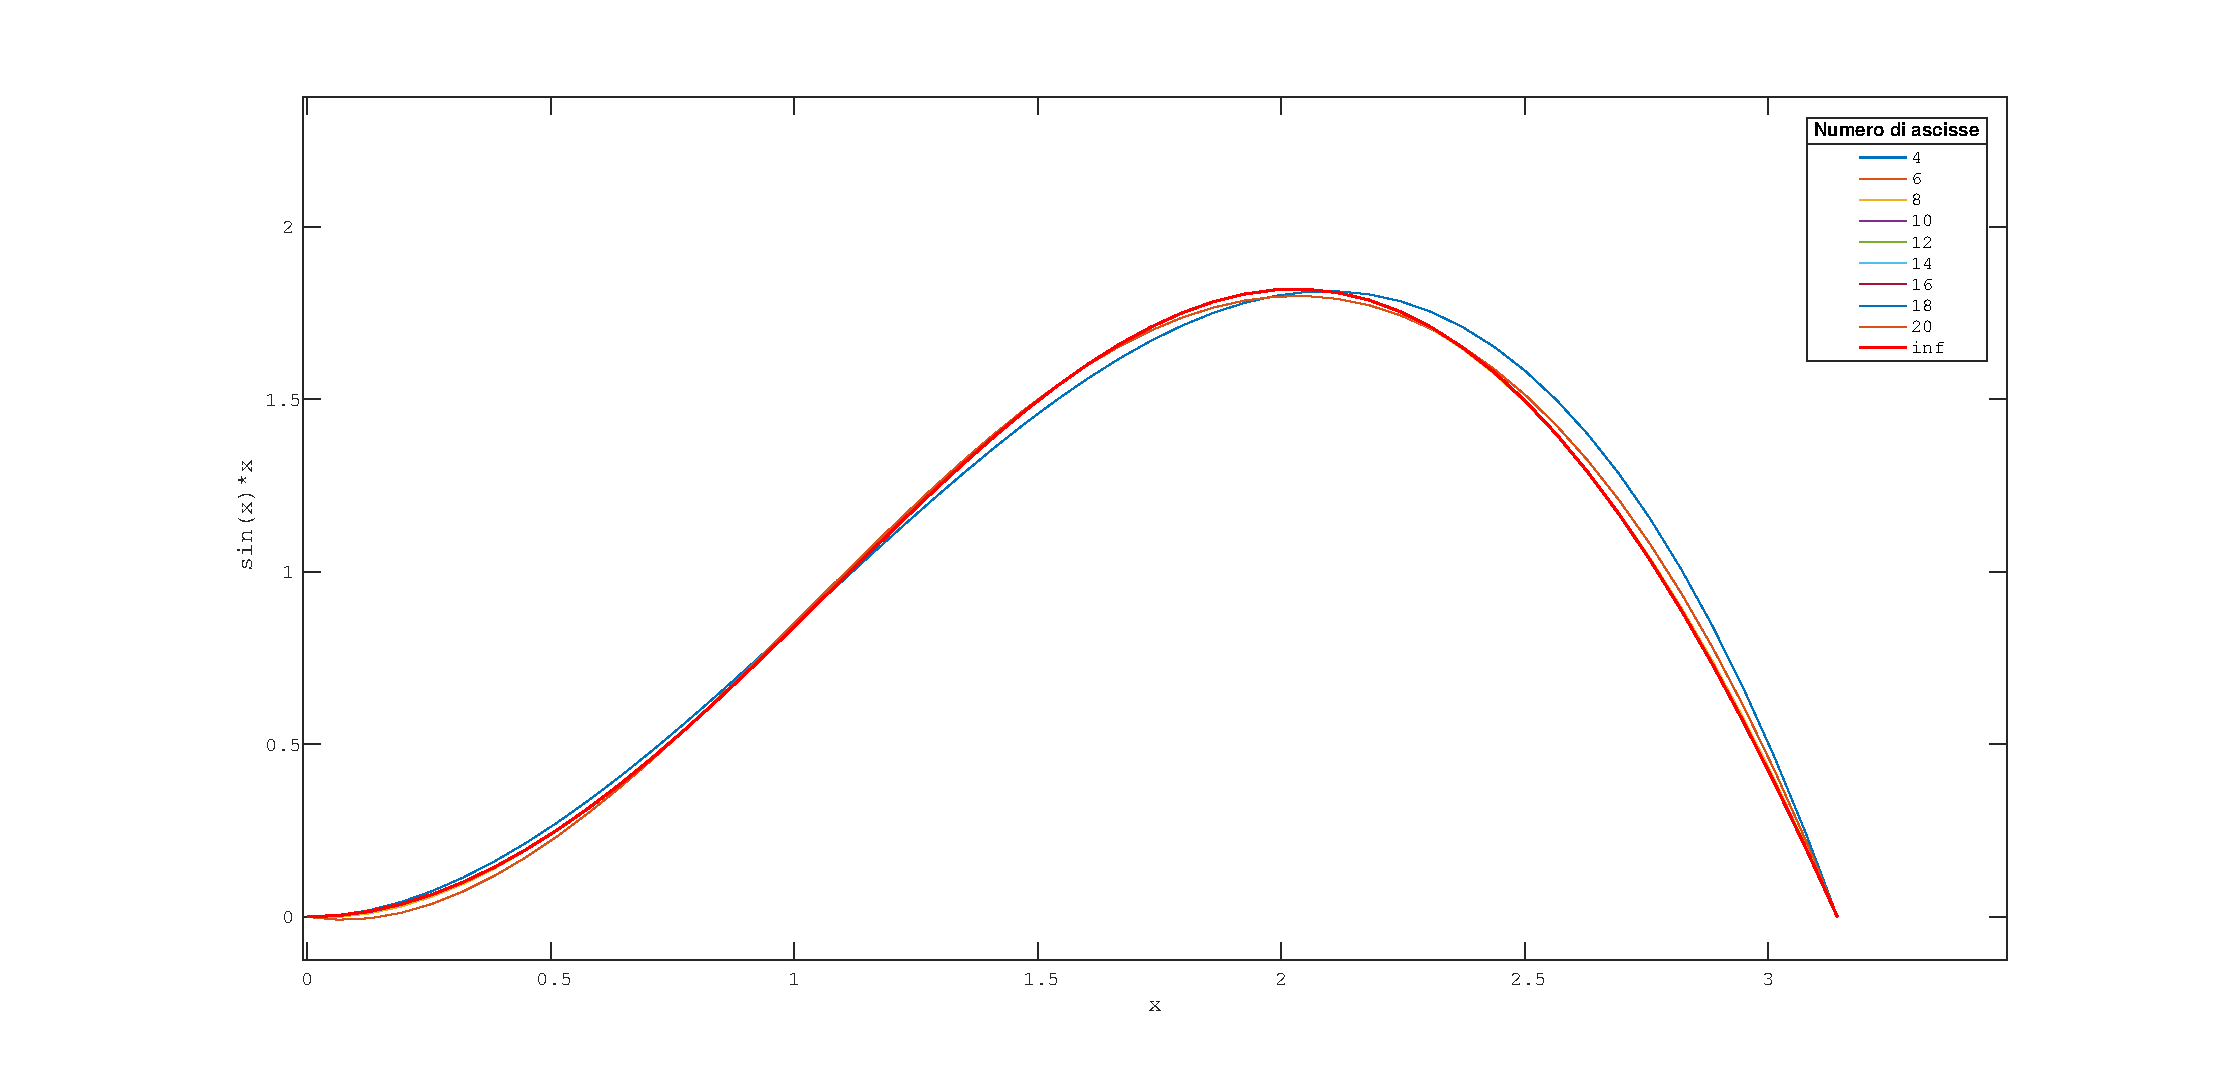
\includegraphics[width=\textwidth]{cap_4/es5/sin_nak}
\caption{$xsin(x)$ interpolata con spline not-a-knot}
\label{plot_sin_nak}
\end{figure}

\begin{figure}
\includegraphics[width=\textwidth]{cap_4/es10/untitled}
\caption{Confronto dei due grafici dell'esercizio 4.8}
\label{fitting}
\end{figure}

%CAP 5 e 6
\begin{figure}
\includegraphics[width=\textwidth]{cap_5_6/es2/error.png}
\caption{Andamento dell'errore per i metodi di Quadratura}
\label{QuadrErr}
\end{figure}
\begin{figure}
\includegraphics[width=\textwidth]{cap_5_6/es2/rapp_err.png}
\caption{Andamento del Rapporto tra gli errori per i metodi di Quadratura}
\label{QuadrRapp}
\end{figure}

\begin{figure}
\includegraphics[width=\textwidth]{cap_5_6/es6/comparison}
\caption{Comparazione dei vari metodi per il calcolo dell'autovettore dominante del PageRank}
\label{PR_comparison}
\end{figure}
